\documentclass[11pt,a4paper]{amsart}

\usepackage[T1]{fontenc}
\usepackage{lmodern}
\usepackage[english]{babel}

\usepackage{amsmath, amssymb, amsthm}
\usepackage{hyperref}
\usepackage{enumerate}
\usepackage{geometry}
\usepackage{float}
\usepackage{csquotes}
\usepackage[ruled,vlined]{algorithm2e}
\SetKwInput{KwIn}{Input}
\SetKwInput{KwOut}{Output}
\SetAlgoSkip{medskip}

\theoremstyle{plain}
\newtheorem{theorem}{Theorem}
\newtheorem{lemma}[theorem]{Lemma}
\newtheorem{proposition}[theorem]{Proposition}
\newtheorem{corollary}[theorem]{Corollary}

\theoremstyle{definition}
\newtheorem{definition}{Definition}

\theoremstyle{remark}
\newtheorem{remark}{Remark}

\usepackage[
    backend=biber,
    style=numeric,
    sorting=none
]{biblatex}
\addbibresource{bibliography.bib}

\usepackage{tikz}
\usetikzlibrary{
  calc,
  intersections,
  arrows.meta,
  decorations.pathreplacing,
  patterns,
  positioning
}

\geometry{margin=2.8cm}

\title{Nested Radicals of {Ramanujan}'s Type with Arbitrary Coefficient Sequences}
\author{Artur Flamandzki}
\thanks{Email address: \texttt{flamandzki.artur@gmail.com}}
\date{\today}


\begin{document}

\begin{abstract}
The classical infinite nested radical of Ramanujan admits numerous variations and generalizations, many of which have been studied independently in the literature. In this paper, we present a unified framework for nested radicals of Ramanujan type by allowing the coefficients to be generated by an arbitrary real-valued sequence. Starting from the classical construction, we show that several known generalizations, including parametric and higher-order variants, arise naturally as special cases of this approach. Sufficient conditions ensuring real-valuedness and convergence are established for broad classes of coefficient sequences, including non-monotone and oscillatory cases. We further extend the convergence theory beyond the bounded-coefficient setting to a specific unbounded, linearly growing family that contains the classical radical itself, proving exact convergence via a functional-equation argument, we exhibit a constant-coefficient construction converging to an arbitrary prescribed target with an explicit geometric rate, and we prove an arbitrary-profile theorem giving an explicit error bound and exact convergence whenever the reciprocals of the profile have a divergent sum. The proposed formulation provides a structural perspective on nested radicals, emphasizing the role of the underlying coefficient sequence rather than individual ad hoc constructions. All main results have been formally verified in Lean~4/Mathlib.
\end{abstract}

\maketitle

\section{Introduction}

Infinite nested radicals have attracted sustained interest since the seminal examples introduced by Ramanujan~\cite{RamanujanNotebooks}. Among these, the classical radical
\[
R = \sqrt{1 + 2\sqrt{1 + 3\sqrt{1 + 4\sqrt{1 + \cdots}}}} = 3
\]
occupies a central position, both for its elegant closed-form value and for the striking manner in which simple arithmetic progressions appear inside a highly nonlinear expression. This construction has since served as a point of departure for numerous investigations into convergence, generalizations, and structural variations of nested radicals.

Several authors have proposed extensions of Ramanujan’s original idea in different directions. Generalizations to higher-order roots, parametric families, and alternative recursive schemes have been developed, often with the goal of producing prescribed limit values or exploring new analytic identities. While these approaches differ in technical realization, they share a common feature: each introduces a specific modification of the coefficients appearing in the recursive structure of the radical.

Despite the variety of known constructions, a unifying viewpoint has remained implicit. Existing works typically focus on particular families of coefficients or on individual transformations of the classical form, rather than on the underlying mechanism governing nested radicals as a whole. As a consequence, different generalizations are usually treated as separate phenomena, even when they exhibit closely related behavior.

The present paper proposes a simple and general framework that subsumes many of these constructions. Starting from the classical Ramanujan radical, we consider nested radicals defined by a recursion of the form
\[
R_k = \sqrt{1 + a_k R_{k+1}},
\]
where the coefficients \(a_k\) are generated by an arbitrary real-valued sequence. This perspective allows the classical example, as well as several known generalizations from the literature, to be recovered as special cases corresponding to particular choices of the sequence \((a_k)\).

Within this framework, the emphasis shifts from individual closed-form identities to structural properties of the coefficient sequence. We derive sufficient conditions ensuring real-valuedness and convergence of the resulting nested radicals and show that these conditions are flexible enough to accommodate monotone, non-monotone, and oscillatory sequences. We also show that convergence can be established beyond the bounded-coefficient setting for a specific unbounded, linearly growing family containing the classical radical, and we exhibit a constant-coefficient construction reaching an arbitrary prescribed target exactly. A final result treats arbitrary profiles: for any positive sequence $(R_k)$ with $R_k\ge 1$ and the coefficients that make it satisfy the recursion exactly, the truncations converge to $R_1$ whenever $\sum 1/R_k$ diverges, with an explicit bound on the error. This makes it possible to systematically construct and analyze broad families of Ramanujan-type radicals within a single coherent setting.

The paper is organized as follows. Section~\ref{sec:related} reviews several representative constructions of Ramanujan-type nested radicals from the literature. The motivation and conceptual origin of the general framework are discussed in Section~\ref{sec:motivation}. The general formulation with arbitrary coefficient sequences, together with basic convergence results and their extension to specific unbounded families, is presented in Section~\ref{sec:general-framework}. Known constructions are embedded into the proposed framework in Section~\ref{sec:embedding}. Section~\ref{sec:formal-verification} summarizes the accompanying formal verification. Final remarks and possible directions for further investigation are given in the concluding section.

\section{Related Constructions of Ramanujan-Type Nested Radicals}
\label{sec:related}

Several generalizations of Ramanujan’s classical nested radical have appeared in the literature, differing mainly in the choice of coefficients and the form of the recursive relation. In this section, we briefly review a small selection of representative constructions that are most closely related to the present work. The emphasis is placed on their structural form and scope rather than on technical details, which may be found in the original references.

\subsection{Higher-Order and Parametric Variants}
\label{subsec:higher-order-parametric}

One direction of generalization replaces the square root in Ramanujan’s construction by higher-order roots. Such variants preserve the recursive nature of the radical while modifying the nonlinear operation at each level. These constructions typically lead to families of nested radicals whose convergence properties depend on both the order of the root and the chosen coefficients. While this approach enlarges the class of admissible radicals, the coefficients are usually restricted to specific functional forms in order to retain analytic tractability.

Another line of work introduces parametric schemes in which the coefficients are adjusted so as to achieve prescribed limiting values. In these constructions, parameters are chosen to control the growth or decay of the nested radical, allowing the resulting expression to converge to a desired real number. This perspective emphasizes the inverse problem of nested radicals, namely the reconstruction of coefficients from target limits, but generally relies on particular parameterizations rather than a fully flexible coefficient sequence.

\subsection{Alternative Recursive and Algebraic Variants}
\label{subsec:alternative-recursive}

Further variations arise from modifications of the recursive relation itself or from algebraic manipulations of the classical Ramanujan radical. These include constructions based on alternative nesting patterns, algebraic identities, or rearrangements that preserve convergence while producing new explicit forms. Such variants often highlight elegant identities and special cases, illustrating the richness of Ramanujan-type expressions.

Although these approaches differ in motivation and technique, they share a common feature: each focuses on a specific family of coefficients or recursive forms, tailored to the construction at hand. As a result, the resulting generalizations are typically studied in isolation, without an explicit framework that accommodates arbitrary coefficient sequences within a single unifying formulation.


\section{Motivation and Conceptual Origin of the General Framework}
\label{sec:motivation}

The general formulation presented in this paper arose from an attempt to identify a common structural principle underlying several known constructions of Ramanujan-type nested radicals. Rather than introducing a new isolated example, the goal was to understand which features of the classical radical are essential and which may be varied without destroying convergence or real-valuedness.

A key observation is that the defining recursion of Ramanujan’s nested radical naturally separates two distinct components. On the one hand, there is the nonlinear operation of taking square roots, which remains fixed throughout the construction. On the other hand, there is the sequence of coefficients appearing inside the radical, which encodes the arithmetic structure driving the recursion. In the classical example, these coefficients form a simple arithmetic progression, while in later generalizations they are modified in various ad hoc ways.

\subsection*{Reverse Construction as a Guiding Principle.}
Classical treatments of nested radicals typically adopt a forward-evaluation perspective: successive truncations are computed by extending the radical deeper and observing the convergence of the resulting values. From this point of view, the nested radical is evaluated as a static expression whose limit is approached asymptotically.

In contrast, the present work is guided by a reversed perspective. Instead of evaluating the radical forward and inspecting its limit, one may prescribe a desired value at the first level of the recursion and ask what continuation of the radical is required in order for this boundary condition to be satisfied exactly. This backward or rolling viewpoint shifts attention from passive evaluation to structural adjustment of the recursive tail, revealing the nested radical as a system that can be tuned rather than merely observed.

\subsection*{Backward Perspective and Convergence Behavior.}
Viewing the nested radical from this backward perspective also offers an intuitive interpretation of its convergence properties. By adjusting the tail of the recursion to meet a prescribed condition at the root, control over the global behavior of the radical is effectively transferred to the deeper levels of the construction. In this setting, convergence is no longer an incidental outcome of repeated forward evaluation, but a property that can be influenced through suitable constraints on the recursive continuation.

This intuition naturally leads to the introduction of admissibility or safety conditions on the coefficients. Such conditions ensure that the backward adjustment of the tail remains within the realm of real-valued expressions and that the recursive process does not destabilize. From this viewpoint, convergence criteria emerge as structural safeguards that guarantee the consistency of the backward construction.

\subsection*{From Reverse Construction to Arbitrary Coefficient Sequences.}
Once the nested radical is interpreted as a structure whose tail may be designed to satisfy a prescribed boundary condition, the role of the coefficients changes fundamentally. Rather than being fixed numerical inputs, the coefficients become the primary objects through which the behavior of the radical is controlled. This shift motivates the abstraction of the coefficients into an independent generating sequence.

Consequently, it becomes natural to consider nested radicals defined by arbitrary coefficient sequences \( a_k = f(k) \), subject to basic admissibility conditions ensuring real-valuedness and convergence. From this perspective, many existing constructions may be viewed as particular realizations of a more general mechanism, distinguished mainly by their choice of generating sequence. This observation provides the conceptual bridge from the backward construction principle to the general framework developed in the subsequent sections.

\section{General Formulation with Arbitrary Coefficient Sequences}
\label{sec:general-framework}

We now introduce the general framework for nested radicals of Ramanujan type. Let $(a_k)_{k \geq 1}$ be a real-valued sequence and define a nested radical recursively by
\[
R_k = \sqrt{1 + a_k R_{k+1}}, \qquad k \geq 1.
\]
For a fixed truncation depth $N$, the corresponding truncated radical is given by
\[
R_1^{(N)} = \sqrt{1 + a_1 \sqrt{1 + a_2 \sqrt{\,\cdots\, \sqrt{1 + a_N}}}}.
\]
The object of interest is the behavior of $R_1^{(N)}$ as $N \to \infty$ and the existence of a finite real limit.

\subsection{Existence and Convergence Criteria}
\label{subsec:existence-convergence}

We first establish simple sufficient conditions ensuring that the recursion is well defined and that the sequence of truncated radicals converges. A full necessary-and-sufficient criterion for convergence of a general infinite nested radical $\sqrt{a_1+\sqrt{a_2+\sqrt{a_3+\cdots}}}$ was established by Herschfeld~\cite{Herschfeld1935}: convergence holds if and only if $a_n^{2^{-n}}$ is bounded. The condition adopted here is a simple special case tailored to the bounded-coefficient setting of this framework, not a restatement of that general result. Assume that the coefficient sequence $(a_k)$ satisfies
\[
a_k \geq 0 \qquad \text{for all } k \geq 1.
\]
Under this assumption, the recursion produces a sequence of nonnegative real numbers and the truncated values $R_1^{(N)}$ form a monotone increasing sequence in $N$.

Moreover, if the coefficients are uniformly bounded, that is,
\[
0 \leq a_k \leq A \qquad \text{for all } k \geq 1
\]
for some constant $A > 0$, then the sequence $(R_1^{(N)})_{N \geq 1}$ is bounded from above. Indeed, a straightforward induction shows that
\[
R_1^{(N)} \leq r^{\ast} := \frac{A + \sqrt{A^2 + 4}}{2},
\]
which implies convergence of the truncated radicals to a finite real limit. (The nonnegativity assumption $a_k \ge 0$ is in fact only needed for monotonicity: the upper bound $R_1^{(N)} \le r^\ast$ itself follows from $a_k \le A$ alone, regardless of sign.)

The above assumptions are sufficient but not necessary. In particular, the framework admits a controlled relaxation of the nonnegativity condition on the coefficients, provided the recursion remains real-valued.

\begin{lemma}[Controlled negative coefficients]
\label{lem:controlled-negativity}
Let $(a_k)$ be a real-valued sequence such that
\[
-A_- \leq a_k \leq A \qquad \text{for all } k \geq 1,
\]
with constants $A \geq 0$ and $A_- \geq 0$. Suppose that the bound
\[
A_- \leq \frac{2}{A + \sqrt{A^2 + 4}}
\]
holds. Then the recursion
\[
R_k = \sqrt{1 + a_k R_{k+1}}
\]
is well defined in $\mathbb{R}$ for all truncation depths $N$, and the corresponding sequence of truncated radicals $(R_1^{(N)})_{N \geq 1}$ is bounded.
\end{lemma}

\begin{proof}
The condition ensures that the radicand $1 + a_k R_{k+1}$ remains nonnegative for all admissible values of $R_{k+1}$ bounded by $r^{\ast}$. An inductive argument shows that the recursion does not leave the real domain and that the truncated radicals remain uniformly bounded. \qed
\end{proof}

This lemma formalizes the notion of \emph{controlled negativity}: small negative values of the coefficients are admissible as long as they do not destabilize the recursive structure. Such conditions act as safety constraints ensuring real-valuedness and convergence, while significantly enlarging the class of admissible coefficient sequences.

\subsection{Convergence for an Unbounded, Linearly Growing Family}
\label{subsec:unbounded-linear}

The sufficient conditions of Section~\ref{subsec:existence-convergence} require a fixed ceiling $A$ with $a_k \le A$ for all $k$. This excludes coefficient sequences that grow without bound — including, notably, the classical case itself (Section~\ref{subsec:classical-ramanujan}). We now establish convergence for a specific unbounded, linearly growing family that contains the classical radical as a special case, resolving that attribution.

For an integer target $N \ge 2$, consider the coefficient sequence
\[
a_k = N + k - 2, \qquad k \ge 1,
\]
already introduced in Appendix~\ref{app:numerical} as the coefficients underlying the identity chain of Algorithm~\ref{alg:identity}. Write $R_1^{(d)}(N)$ for the depth-$d$ truncation of this family, using the same convention as the main definition of $R_1^{(N)}$ above (the innermost term is $\sqrt{1+a_d}$, i.e. a virtual seed of $1$) — this is distinct from the separate tail-zero "forward evaluation" convention used for numerical illustration in Algorithm~\ref{alg:forward}.

\begin{proposition}[Moving-ceiling boundedness]
\label{prop:moving-ceiling}
For every integer $N \ge 2$ and every depth $d \ge 0$, $0 \le R_1^{(d)}(N) \le N$.
\end{proposition}

\begin{proof}
By induction on $d$. The case $d=0$ is immediate ($R_1^{(0)}(N) = 1 \le N$). For the inductive step, removing the outermost layer of $R_1^{(d+1)}(N)$ exposes exactly the depth-$d$ truncation of the same family with target $N+1$ in place of $N$:
\[
R_1^{(d+1)}(N) = \sqrt{1+(N-1)\,R_1^{(d)}(N+1)}.
\]
By the inductive hypothesis applied to $N+1$, $R_1^{(d)}(N+1) \le N+1$, so
\[
R_1^{(d+1)}(N) \le \sqrt{1+(N-1)(N+1)} = \sqrt{N^2} = N. \qedhere
\]
\end{proof}

Unlike the bound of Section~\ref{subsec:existence-convergence}, the ceiling here is not a fixed constant but moves with the target $N$ itself. Combined with monotonicity in $d$ (which holds unconditionally for $a_k \ge 0$, as in Section~\ref{subsec:existence-convergence}), Proposition~\ref{prop:moving-ceiling} already shows that $R_1^{(d)}(N)$ converges, as $d \to \infty$, to some finite limit $L(N) \le N$.

\begin{theorem}[Exact convergence]
\label{thm:exact-convergence}
For every integer $N \ge 2$, $L(N) = N$.
\end{theorem}

\begin{proof}[Proof sketch]
Passing the identity of Proposition~\ref{prop:moving-ceiling} to the limit $d \to \infty$ on both sides gives the functional equation
\[
L(N) = \sqrt{1 + (N-1)\, L(N+1)}.
\]
Writing $\delta(N) := N - L(N) \ge 0$ for the deficit, squaring the functional equation and simplifying (using $(N-1)(N+1)=N^2-1$) yields the exact recursion
\[
\delta(N+1) = \delta(N)\cdot \frac{2N - \delta(N)}{N-1}.
\]
Since $R_1^{(1)}(N) = \sqrt{1+a_1} = \sqrt{N} \ge 1$ for $N \ge 2$ and $L(N) \ge R_1^{(1)}(N)$ by monotonicity, we have $\delta(N) \le N-1$ for every $N$; substituting this ceiling into the recursion gives the unconditional bound
\[
\delta(N+1) \ge \delta(N)\cdot \frac{N+1}{N-1},
\]
valid for every $N \ge 2$ — with no restriction to small $\delta$, and no arbitrary cutoff. Telescoping this bound over $j$ steps from a fixed $N_0$ gives
\[
\delta(N_0+j) \ge \delta(N_0)\cdot \frac{(N_0+j)(N_0+j-1)}{N_0(N_0-1)},
\]
a lower bound growing quadratically in $j$. If $\delta(N_0) > 0$ for some $N_0$, this quadratic lower bound eventually exceeds the linear ceiling $\delta(N_0+j) \le N_0+j-1$ established above — a contradiction reached after finitely many steps for any positive starting deficit. Hence $\delta(N) = 0$ for every $N \ge 2$. \qedhere
\end{proof}

Theorem~\ref{thm:exact-convergence} resolves, for this family, a claim that Section~\ref{subsec:classical-ramanujan} previously attributed without proof to the boundedness result of Section~\ref{subsec:existence-convergence}: that attribution does not literally hold, since $a_k = N+k-2$ has no fixed ceiling, but the exact convergence itself is correct, and Theorem~\ref{thm:exact-convergence} supplies the missing argument. The proof is a self-contained argument specific to this family, not an application of Herschfeld's general criterion~\cite{Herschfeld1935}; its structure — a global growth-rate bound forcing a contradiction rather than a direct estimate — is nonetheless in the same spirit as that classical approach to convergence of infinite nested radicals. Taking $N=3$ recovers the classical Ramanujan radical; taking $N=2$ recovers the sequence $a_k=k$. All statements in this subsection have been formally verified in Lean~4/Mathlib; see Section~\ref{sec:formal-verification}.

\subsection{A Constant-Coefficient Family with Exact, Explicit Convergence}
\label{subsec:target-radical}

The boundedness machinery of Section~\ref{subsec:existence-convergence} is normally applied to obtain an upper bound $r^\ast$ on the radical; the same machinery can equally be used to \emph{design} a coefficient sequence hitting a prescribed target exactly. For a target $t \ge 1$, let
\[
a_k = t - \frac{1}{t} \qquad \text{for every } k \ge 1
\]
be a \emph{constant} coefficient sequence. A direct computation shows that $t$ is itself the fixed point of $x \mapsto \sqrt{1+Ax}$ for $A = t-1/t$, i.e. $r^\ast = t$, so Section~\ref{subsec:existence-convergence} already guarantees $R_1^{(d)} \le t$ for every depth $d$.

\begin{proposition}
\label{prop:target-radical}
With $a_k = t - 1/t$ for all $k$, $R_1^{(d)} \to t$ as $d \to \infty$, and the convergence is geometric: writing $\rho = (t-1/t)/t = 1 - 1/t^2 < 1$,
\[
t - R_1^{(d)} \le \rho^{\,d}\,(t - T),
\]
where $T$ denotes the seed value at depth $0$.
\end{proposition}

\begin{proof}[Proof sketch]
The gap $e_d := t - R_1^{(d)}$ satisfies, via the conjugate identity
\[
t - \sqrt{t^2 - A e_d} = \frac{A e_d}{t + \sqrt{t^2 - Ae_d}}
\]
together with $R_1^{(d+1)} \ge 0$, the one-step bound $e_{d+1} \le \rho\, e_d$; iterating gives the stated geometric bound. \qedhere
\end{proof}

Proposition~\ref{prop:target-radical} gives a construction of a nested radical converging exactly to a prescribed target $t$ with a single constant coefficient. For $t=3$, the bound above gives ratio $\rho = 8/9$, while the true asymptotic rate is $A/(2t) = 4/9$ (the derivative of the fixed-point map at $t$). The coefficient rule differs from that of Ramanujan's radical, so this is a separate construction within the same general framework.

This construction generalizes to any root order $n\ge 2$: it only solves the single fixed-point equation $1+A\cdot t=t^n$ for one constant $A=(t^n-1)/t$, so the factorization question that arises for the exact-value problem of unbounded families at $n\ge 3$ (Section~\ref{subsec:higher-order-roots}) does not occur here. Formally verified in Lean~4 (Section~\ref{sec:formal-verification}): for every root order $n\ge 2$, the recursion $R_k=(1+A R_{k+1})^{1/n}$ with $A=(t^n-1)/t$ converges to $t$ exactly, with a geometric bound $\rho_n=1-1/t^n$ generalizing the $n=2$ ratio above.

\subsection{Arbitrary Profiles: an Explicit Error Bound}
\label{subsec:profile}

Algorithm~\ref{alg:design_gen} prescribes a positive sequence $(R_k)$ and computes the coefficients that make it satisfy the recursion exactly. The following theorem states what this gives for the truncations with the standard seed $1$, for an arbitrary profile and any root order $n\ge 2$. Write $T_d$ for the depth-$d$ truncation with seed $1$,
\[
T_d=\Bigl(1+a_1\bigl(1+a_2\bigl(\cdots(1+a_d\cdot 1)^{1/n}\cdots\bigr)^{1/n}\bigr)^{1/n}\Bigr)^{1/n},\qquad T_0=1 .
\]

\begin{theorem}[Arbitrary profile]
\label{thm:profile}
Let $n\ge 2$, let $R_k\ge 1$ for all $k\ge 1$, and let $(a_k)$ satisfy $R_k^{\,n}=1+a_kR_{k+1}$ for all $k\ge 1$. Then $a_k\ge 0$ and, for every $d\ge 0$,
\[
0\;\le\; R_1-T_d\;\le\; R_1\prod_{j=1}^{d}\Bigl(1-\frac1{R_j}\Bigr).
\]
In particular, if $\sum_{k}1/R_k$ diverges, then $T_d\to R_1$ as $d\to\infty$.
\end{theorem}

\begin{proof}
Since $a_k=(R_k^n-1)/R_{k+1}$ and $R_k,R_{k+1}\ge 1$, we have $a_k\ge 0$, so every radicand is at least $1$ and $T_d\ge 1$ for all $d$ and all shifted profiles.

Fix a profile $(R_k)$ and let $s=T_{d+1}$ and $u=T_d'$, where $T_d'$ denotes the depth-$d$ truncation of the shifted problem (profile $(R_{k+1})_{k\ge 1}$, coefficients $(a_{k+1})_{k\ge 1}$). Then $s^n=1+a_1u$ and $R_1^n=1+a_1R_2$, so
\[
R_1^n-s^n=a_1(R_2-u)=\frac{R_1^n-1}{R_2}\,(R_2-u).
\]
On the other hand $R_1^n-s^n=(R_1-s)\sum_{i=0}^{n-1}R_1^{\,i}s^{\,n-1-i}$, and since $s\ge 1$ the sum is at least $\sum_{i=0}^{n-1}R_1^{\,i}=(R_1^n-1)/(R_1-1)$ (for $R_1>1$; if $R_1=1$ then $a_1=0$ and $T_{d+1}=1=R_1$). Dividing gives
\[
R_1-T_{d+1}\;\le\;\frac{R_1-1}{R_2}\,\bigl(R_2-T_d'\bigr).
\]
Define $e_d(R)=R_1-T_d$ for the profile $R=(R_k)$. By induction on $d$, applied to all shifts of the profile simultaneously,
\[
e_d(R)\le \prod_{j=1}^{d}\frac{R_j-1}{R_{j+1}}\cdot(R_{d+1}-1)
= R_1\prod_{j=1}^{d}\Bigl(1-\frac1{R_j}\Bigr)\Bigl(1-\frac1{R_{d+1}}\Bigr)\le R_1\prod_{j=1}^{d}\Bigl(1-\frac1{R_j}\Bigr),
\]
where the base case is $e_0(R)=R_1-1$. Nonnegativity $R_1-T_d\ge 0$ follows from the same one-step identity, since $s\le R_1$ whenever $u\le R_2$. Finally $1-x\le e^{-x}$ gives $\prod_{j\le d}(1-1/R_j)\le\exp(-\sum_{j\le d}1/R_j)$, which tends to $0$ when $\sum 1/R_k$ diverges. \qedhere
\end{proof}

No limit object, functional equation or deficit-growth argument is used. Three special cases are instructive.

\begin{itemize}
\item \emph{Constant profile.} For $R_k=t\ge 1$ we have $a_k=(t^n-1)/t$, the coefficient of Section~\ref{subsec:target-radical}, and the bound reads $t-T_d\le t(1-1/t)^d$.
\item \emph{The classical family, $n=2$.} For $R_k=N+k-1$ the coefficients are $a_k=(R_k^2-1)/R_{k+1}=N+k-2$. Here $\prod_{j=1}^d(1-1/R_j)=(N-1)/(N+d-1)$, so $N-T_d\le N(N-1)/(N+d-1)$, and $\sum 1/R_k$ diverges. This recovers Theorem~\ref{thm:exact-convergence} for $n=2$ together with an explicit rate.
\item \emph{The classical family, even $n$.} For even $n$ the same profile gives $a_k=\mathrm{altSum}_n(R_k)=(R_k^n-1)/(R_k+1)$ with $\mathrm{altSum}_n(x)=\sum_{i=0}^{n-1}(-1)^{n-1-i}x^i$, and the theorem again gives convergence to $N$.
\end{itemize}

For odd $n$ the classical family has radicand $-1+a_kR_{k+1}$ rather than $1+a_kR_{k+1}$, so it is outside the scope of Theorem~\ref{thm:profile}; its exact value is obtained by the deficit-growth argument of Section~\ref{subsec:higher-order-roots}. Theorem~\ref{thm:profile} is formally verified in Lean~4 (Section~\ref{sec:formal-verification}).

\subsection{Structural Properties and Bounds}
\label{subsec:structural-bounds}

Within the general framework, the qualitative behavior of the nested radical is governed primarily by the structure of the coefficient sequence $(a_k)$. Growth, oscillation, and clustering properties of the coefficients are reflected in the rate of convergence and in the limiting value of the radical.

The bound $r^{\ast}$ provides a universal upper estimate depending only on the supremum of the coefficients and is independent of their detailed distribution. This highlights the robustness of the construction and explains why a wide variety of coefficient sequences lead to well-defined Ramanujan-type nested radicals.

In particular, Lemma~\ref{lem:controlled-negativity} shows that this robustness extends beyond the nonnegative setting: controlled negative values of the coefficients may be admitted without destabilizing the recursion. Sections~\ref{subsec:unbounded-linear} and~\ref{subsec:target-radical} show, further, that robustness extends beyond the bounded setting as well, for suitably structured unbounded or constant families. This demonstrates that stability is a structural property of the recursive operator rather than a consequence of monotonicity or boundedness of the coefficients alone.

From a numerical perspective, this distinction is also reflected in the convergence behavior of different evaluation strategies. While the classical forward evaluation exhibits slow convergence, as illustrated in Table~\ref{tab:ramanujan-forward}, the backward construction eliminates this numerical deficit by enforcing structural consistency at each truncation level. This observation further supports the interpretation of stability as an intrinsic property of the recursive operator rather than an artifact of forward approximation.

The formulation presented here emphasizes that the recursive square-root structure acts as a stable nonlinear operator, while the coefficient sequence serves as the primary carrier of arithmetic or structural information. This viewpoint will be used in the next section to embed several known constructions into the present framework.

\section{Embedding Known Constructions into the General Framework}
\label{sec:embedding}

In this section we show that several well-known constructions of Ramanujan-type nested radicals appearing in the literature arise naturally as special cases of the general formulation introduced above. Each construction is first recalled in its original form, following the presentation of the respective authors, and is then interpreted within the present framework by identifying the corresponding coefficient sequence.

\begin{figure}[H]
\centering
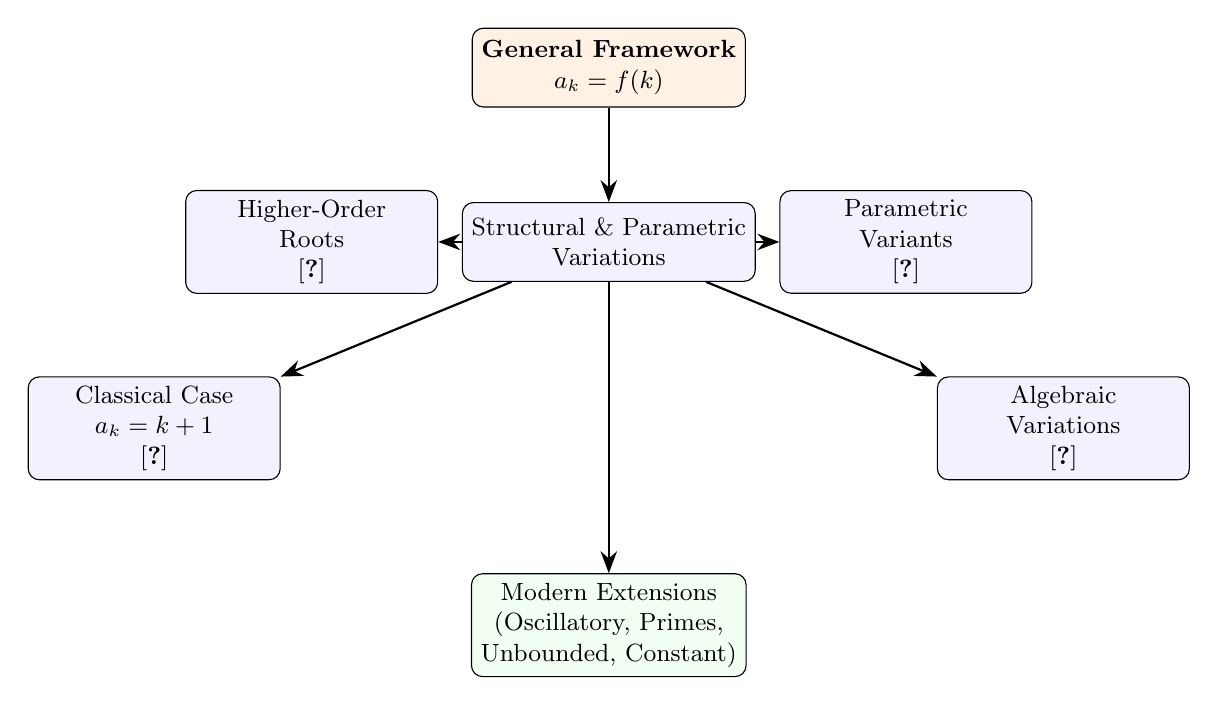
\begin{tikzpicture}[
    node distance = 1.2cm and 0.8cm,
    box/.style = {draw, rectangle, rounded corners, minimum width=3.2cm, minimum height=1cm, align=center, fill=blue!5, font=\small},
    arrow/.style = {thick, -{Stealth[scale=1.2]}}
]

% Nodes
\node (top) [box, fill=orange!10] {\textbf{General Framework} \\ $a_k = f(k)$};

\node (mid) [box, below=of top] {Structural \& Parametric \\ Variations};

% Poziom autorów
\node (ramanujan) [box, below left=of mid, xshift=-1.5cm] {Classical Case \\ $a_k = k+1$ \\ \cite{RamanujanNotebooks}};

\node (mitra) [box, left=of mid, xshift=0.5cm] {Higher-Order \\ Roots \\ \cite{MitraNestedRadicals}};

\node (kusniec) [box, right=of mid, xshift=-0.5cm] {Parametric \\ Variants \\ \cite{KusniecRadiciators}};

\node (campbell) [box, below right=of mid, xshift=1.5cm] {Algebraic \\ Variations \\ \cite{CampbellZujevRadicals}};

\node (special) [box, below=of mid, yshift=-2.5cm, fill=green!5] {Modern Extensions \\ (Oscillatory, Primes,\\ Unbounded, Constant)};

% Connections
\draw [arrow] (top) -- (mid);
\draw [arrow] (mid) -- (ramanujan);
\draw [arrow] (mid) -- (mitra);
\draw [arrow] (mid) -- (kusniec);
\draw [arrow] (mid) -- (campbell);
\draw [arrow] (mid) -- (special);

\end{tikzpicture}
\caption{Expanded structural hierarchy: the general framework $a_k = f(k)$ subsuming classical results and modern variations.}
\label{fig:hierarchy_expanded}
\end{figure}

\subsection{The Classical Ramanujan Radical}
\label{subsec:classical-ramanujan}

The classical infinite nested radical introduced by Ramanujan~\cite{RamanujanNotebooks} is given by
\[
R = \sqrt{1 + 2\sqrt{1 + 3\sqrt{1 + 4\sqrt{1 + \cdots}}}} = 3,
\]
and represents one of the most celebrated examples of such constructions. This radical has been studied extensively and serves as a canonical starting point for many later generalizations.

In the notation adopted in this paper, the classical Ramanujan radical corresponds to the coefficient sequence
\[
a_k = k+1, \qquad k \geq 1,
\]
i.e. it is the instance $N=3$ of the family $a_k = N+k-2$ already introduced via the identity chain of Algorithm~\ref{alg:identity}. Thus, the original construction appears as a particular instance of the general recursion
\[
R_k = \sqrt{1 + a_k R_{k+1}},
\]
with a simple arithmetic progression of coefficients. Since $(a_k)$ is unbounded, its convergence does \emph{not} follow directly from the boundedness results of Section~\ref{subsec:existence-convergence} as originally stated there, which require a fixed ceiling $a_k \le A$. Proposition~\ref{prop:moving-ceiling} and Theorem~\ref{thm:exact-convergence} of Section~\ref{subsec:unbounded-linear} supply the missing argument, establishing convergence to exactly $3$ for this family and, more generally, to $N$ for every integer target $N \ge 2$ — which includes the coefficient sequence $a_k = k$ (the case $N=2$) as a further, distinct example, converging to $2$ rather than to the classical value. For square roots the family $a_k=N+k-2$ is Ramanujan's general identity (Entry 4 in~\cite{BerndtNotebooksII}, p.~108, as quoted in~\cite{MitraNestedRadicals}), whose special case is $f(x)=x+1$, so the value $N$ is known; what Theorem~\ref{thm:exact-convergence} supplies is a proof of convergence of the standard truncations by the argument given there.

\subsection{Higher-Order Root Constructions}
\label{subsec:higher-order-roots}

Mitra~\cite{MitraNestedRadicals} treats higher-order roots through the binomial expansion of $(x+1)^n$. Writing $f(x)=x+1$, one has $f(x)^n = 1+\binom n1 x+\dots+\binom n{n-2}x^{n-2} + x^{n-1}f(x+n-1)$, so that the radicand at each level is a full row of Pascal's triangle in the current argument, the argument advances by $n-1$ from one level to the next, and the nested radical takes the form
\[
x+1=\sqrt[n]{1+\tbinom n1 x+\dots+\tbinom n{n-2}x^{n-2}+x^{n-1}\sqrt[n]{\,1+\dots}}.
\]
For $n=2$ this is Ramanujan's family $f(x)=\sqrt{1+x f(x+1)}$. For $n=3$ the convergence is proved there by a boundedness-and-monotonicity argument; for $n\ge 4$ the construction is stated and its evaluation is indicated by the same pattern.

The recursion of the present paper has a different shape: for every root order $n$ the radicand is $1+a_kR_{k+1}$ (or $(-1)^n+a_kR_{k+1}$ in the signed form below), a single coefficient multiplies the next level, and the argument advances by one. For $n=2$ the two descriptions coincide, with $a_k=N+k-2$ and $N=x+1$. For $n\ge 3$ they describe different recursions and the results below do not refer to Mitra's.

The boundedness-and-monotonicity criterion of Section~\ref{subsec:existence-convergence} extends to the operator $R_k = (1+a_k R_{k+1})^{1/n}$ at any fixed root order $n \ge 2$: existence of a finite limit holds for every bounded coefficient sequence $0 \le a_k \le A$. This has been formally verified in Lean~4 (Section~\ref{sec:formal-verification}). The closed-form identity of Algorithm~\ref{alg:identity} and the exact-value question it raises for unbounded families are addressed below.

The moving-ceiling technique of Section~\ref{subsec:unbounded-linear} extends to this operator as well, for the specific unbounded linear family $a_k=N+m(k-2)$, at any fixed root order $n \ge 2$: for $m \ge 1$, existence of a finite limit $L \le N$, with the same key inequality closing the argument at every root order at once; for every $m>0$, the weaker bound $L\le N+1$; and for $0<m\le 1$, the tight shift $L\le N+s(m)$ carries over unchanged from the square-root case (Section~\ref{sec:formal-verification}). The prime-coefficient example (Appendix~\ref{app:nonstandard}) generalizes the same way: the geometric moving-ceiling argument of Section~\ref{sec:formal-verification} transfers to any root order with the identical hypotheses, giving existence of a finite limit for $a_k=p_k$ at every $n\ge 2$.

The classical family $a_k=N+k-2$ itself (Algorithm~\ref{alg:identity}, the case $m=1$ of the moving-ceiling family above) admits a closed-form identity at every root order $n\ge 2$, not only $n=2$: the factor $(x+1)^2-1=x(x+2)$ used at $n=2$ is one instance of the general fact that $x=-1$ is a root of exactly one of $x^n-1$ or $x^n+1$, according to whether $n$ is even or odd, giving in either case a single alternating-sign coefficient polynomial and a closed-form identity $R_k^n=(-1)^n+Q_n(R_k)\cdot R_{k+1}$ with $R_k=N+k-1$, valid for every $n\ge 2$ (verified in Lean~4, Section~\ref{sec:formal-verification}). For even root order, the exact-value closure of Theorem~\ref{thm:exact-convergence} transfers as well: the same deficit-growth argument, applied to this family's own coefficient polynomial in place of the linear $N-1$ used at $n=2$, again forces the limit to equal $N$ exactly, for every even $n\ge 2$. For odd $n$ the same deficit-growth quantity is off by a constant from the even case, so the clean growth ratio picks up an extra per-step shrink factor; this factor is shown to stay bounded away from zero uniformly (via an elementary telescoping-sum estimate and a Weierstrass-type product-sum inequality), which keeps the deficit growth quadratic and forces the limit to equal $N$ exactly for odd $n$ as well. The exact-value closure therefore holds for every $n\ge 2$, both parities (verified in Lean~4, Section~\ref{sec:formal-verification}).

\subsection{Parametric Constructions}
\label{subsec:parametric}

Parametric approaches to nested radicals have been developed by Kusniec~\cite{KusniecRadiciators}, who introduced constructions in which the coefficients are chosen so as to produce prescribed limiting values. In this setting, the nested radical is defined through a recursion of the form
\[
R_k = \sqrt{1 + a_k(\theta)\, R_{k+1}},
\]
where the coefficients depend on one or more parameters $\theta$.

Such constructions fit naturally into the present framework by interpreting the parameter-dependent coefficients as a particular family of generating sequences $(a_k)$. The emphasis in this approach lies on the inverse problem of selecting coefficients to achieve a desired limit, whereas the recursive mechanism itself coincides with the general formulation considered here. Section~\ref{subsec:target-radical} develops one such construction — a constant-coefficient family reaching an arbitrary target exactly — in full detail within the present framework.

Setting $q=1$ in Kusniec's construction recovers the family $a_k = N+k-2$ of Section~\ref{subsec:unbounded-linear} exactly, with $x$ playing the role of $N$. His $n$-th truncation is closed with the exact tail $\sqrt{p_n^2}=p_n=x+n$, so by finite telescoping every such truncation equals $x$, and the identity $\mathcal{R}(x,q)=x$ is read off from this. The truncations with the standard seed, which are the objects of Theorem~\ref{thm:exact-convergence}, are a different sequence. Parameter choices with $q>x$, which make the leading coefficient negative, are checked there case by case.

Kusniec's second (difference-of-oblongs) construction has radicand $q^2+a_k+a_kR_{k+1}$, with an additional term $a_k$ outside the factor multiplying $R_{k+1}$, and coefficients linear in depth with slope $q-1$. It is therefore a different recursion from $R_k=\sqrt{1+a_kR_{k+1}}$ and is not treated here. Separately, existence of a limit for the coefficient sequences $a_k = N+m(k-2)$ of the present recursion, at every slope $m>0$, is established in Section~\ref{sec:formal-verification}.

\subsection{Algebraic and Recursive Variants}
\label{subsec:algebraic-recursive}

Campbell and Zujev~\cite{CampbellZujevRadicals} give new finite nested-radical identities in the manner of Ramanujan's questions to the Indian Mathematical Society, together with methods for constructing such identities. Their work concerns algebraic identities between finite expressions and does not treat infinite nested radicals or their convergence. The authors themselves note the absence of a unifying theory for this body of results: \enquote{there seems no comprehensive theory to cover off the results}~\cite{CampbellZujevRadicals}.

Within the present framework, such variants correspond to specific, often highly structured choices of the coefficient sequence. While their original formulations may obscure this commonality, the general recursion introduced in Section~\ref{sec:general-framework} provides a uniform setting in which these examples can be placed alongside other Ramanujan-type radicals.

\subsection{Summary}

The examples discussed above demonstrate that several classical and modern constructions of nested radicals can be embedded into a single general framework by identifying the appropriate coefficient sequence. This unifying perspective highlights the structural role of the coefficients and clarifies the relationships between constructions that were previously studied independently.

The three works surveyed above vary one feature of the classical radical each: the target value (Kusniec), the choice of algebraic identity (Campbell and Zujev), and the order of the root (Mitra). The framework of this paper varies the coefficient sequence $(a_k)$, and, as formally verified in Lean~4 (Section~\ref{sec:formal-verification}), also the root order for the recursion $R_k^n=1+a_kR_{k+1}$ in the bounded-coefficient case.



\section{Formal Verification}
\label{sec:formal-verification}

The results of Section~\ref{sec:general-framework} — Lemma~\ref{lem:controlled-negativity}, the identity chain of Algorithm~\ref{alg:identity} and its inverse (Algorithm~\ref{alg:design_gen}), the oscillatory example of Appendix~\ref{app:nonstandard}, and the results of Sections~\ref{subsec:unbounded-linear} and~\ref{subsec:target-radical} (Proposition~\ref{prop:moving-ceiling}, Theorem~\ref{thm:exact-convergence}, Proposition~\ref{prop:target-radical}) and Theorem~\ref{thm:profile} — have been formally verified in Lean~4 using Mathlib. The formalization compiles with no admitted (\texttt{sorry}) proof obligations and is available at:
\begin{center}
\url{https://github.com/Flaman55/RamanujanNestedRadicals}
\end{center}
{\sloppy Four of these statements --- exact convergence of the classical family for square roots and for every root order $n \ge 2$, and the explicit error bound and exact convergence of Theorem~\ref{thm:profile} --- are registered in the Palomar registry of Lean-verified results as PALOMAR-2026-10-21-000015 (\url{https://palomar-registry.org/entry?id=PALOMAR-2026-10-21-000015}), whose review checks that the formal statements match the statements of this paper.\par}

The sequence $a_k=k$ is already covered directly, with no reindexing needed: it is exactly the $N=2$ instance of $a_k=N+k-2$, so Theorem~\ref{thm:exact-convergence} applied at $N=2$ gives $a_k=k$ converging to $2$.

The tail-independence discussion of Appendix~\ref{app:numerical-stability} (Table~\ref{tab:tail-independence}) has also been formally verified, closing a claim that had previously only been asserted in prose: the underlying fact is that the truncated radical is monotone not only in the truncation depth (Section~\ref{subsec:existence-convergence}) but also in the tail seed value itself, for nonnegative coefficients. Combined with the exact rolling identity of Algorithm~\ref{alg:identity}, restated at the level of the truncated radical rather than as a pointwise recursion on the closed form, this shows that any tail policy $T(d) \le N+d$ — in particular, all five policies tabulated — yields a truncated radical bounded above by $N$, exactly as claimed.

The prime-coefficient example of Appendix~\ref{app:nonstandard} is also now covered, though only in an existence sense: any coefficient sequence growing at most geometrically ($a_k \le r^k$ for some fixed $r>1$) already admits a depth-independent bound on the truncated radical, via a moving ceiling that closes to a fixed constant. Since $p_k \le 4^k$ — an elementary consequence of Bertrand's postulate — this applies to the primes, giving existence of a finite limit for $a_k=p_k$. Unlike the $a_k=N+k-2$ family above, the exact limiting value is not determined by this argument and remains open.

The family $a_k=N+m(k-2)$ (Section~\ref{subsec:higher-order-roots}) has also been formally verified for every slope $m>0$, not only $m=1$: existence of a finite limit is proved by the same moving-ceiling technique, with the ceiling shifting by $m$ per layer instead of by a fixed constant. For $m \ge 1$ this gives the same bound $L\le N$ as the $m=1$ case; for $0<m\le 1$ the tightest bound obtainable by this technique is $L \le N+s(m)$, where $s(m)=(\sqrt{5m^2+4}-3m)/2$ is the positive root of $s^2+3ms+m^2=1$, matching $L\le N$ exactly at $m=1$. As with the prime-coefficient case, only existence is established for $m\ne 1$; the exact limiting value is known only at $m=1$ (Theorem~\ref{thm:exact-convergence}).

The boundedness, monotonicity and convergence result of Section~\ref{subsec:existence-convergence} has also been formally verified for the higher-order-root operator of Section~\ref{subsec:higher-order-roots}: for the recursion $R_k=(1+a_k R_{k+1})^{1/n}$ at any fixed root order $n \ge 2$, existence of a finite limit is proved for every bounded sequence $0 \le a_k \le A$, via an explicit compatible ceiling $r=A+2$. This covers arbitrary root order together with arbitrary bounded coefficients.

The moving-ceiling technique for the unbounded linear family $a_k=N+m(k-2)$ (above) has likewise been extended to arbitrary root order: for any slope $m \ge 1$ and any fixed $n \ge 2$, existence of a finite limit $L \le N$ is proved for the recursion $R_k=(1+a_k R_{k+1})^{1/n}$, combining the shift-by-$m$ ceiling of the linear family with the arbitrary-root-order machinery above. The key inequality needed ($m \ge 1$) is unchanged across every root order, recovering the $n=2$ case exactly. The same extension covers every slope $m>0$ (bound $L\le N+1$) and, for $0<m\le 1$, the tight shift $L\le N+s(m)$ — in each case the square-root inequality is unaffected by the change of root order, since $(N+c)^n\ge (N+c)^2$ for $N+c\ge 1$ and $n\ge 2$.

The geometric moving-ceiling argument for the prime-coefficient family $a_k=p_k$ (above) extends the same way: the hypothesis $1\le A(A-r^2)$ already forces $A\cdot r^i\ge 1$ for every depth-shift $i$, which is exactly what is needed to pass from the square-root bound to any root order $n\ge 2$, with no change to the constants ($r=4$, $A=17$). The small-amplitude oscillatory family (Appendix~\ref{app:nonstandard}, $0\le\alpha\le 1$) is bounded, so its convergence at any root order is a direct instance of the bounded-coefficient result above, requiring no separate argument.

The classical unbounded family $a_k=N+k-2$ (Algorithm~\ref{alg:identity}, Theorem~\ref{thm:exact-convergence}) has also been formally verified at arbitrary root order, using a single argument that covers both even and odd $n$ by branching only on a sign: $x=-1$ is a root of exactly one of $x^n-1$ or $x^n+1$ according to the parity of $n$, giving in either case an alternating-sign coefficient polynomial $Q_n$ and the exact identity $R_k^n=(-1)^n+Q_n(R_k)\cdot R_{k+1}$ with $R_k=N+k-1$, for every $n\ge 2$ — the case $n=2$ recovers Algorithm~\ref{alg:identity}'s own identity exactly. Existence of a finite limit $L(N)\in[1,N]$ is proved for every $n\ge 2$, both parities (note the seed used here is $1$, not $0$: for odd $n$ the seed $0$ makes the radicand negative, which the seed $1$ avoids). The exact value $L(N)=N$ is proved for every $n\ge 2$, both parities. For even $n$, by the same deficit-growth telescoping argument as Theorem~\ref{thm:exact-convergence} — it transfers with no structural change, since for even $n$ the coefficient polynomial's defining identity supplies exactly the bound the argument needs. For odd $n$, the same factorization instead supplies a bound off by a constant, so the deficit-growth ratio picks up an extra per-step shrink factor relative to the even case; the product of these shrink factors over any number of steps is shown to stay bounded below by a fixed positive constant, uniformly in the starting point and the number of steps, via an elementary telescoping-sum estimate combined with a Weierstrass-type product-sum inequality ($\prod(1-x_i)\ge 1-\sum x_i$) proved directly, with no matching lemma found in Mathlib. This keeps the deficit growth quadratic in the step count, merely scaled by a fixed constant, which still suffices to outpace the linear ceiling in the closing argument — so the odd case closes by the same mechanism as the even one, with one additional ingredient.

The constant-coefficient exact-target radical of Section~\ref{subsec:target-radical} has also been formally verified at every root order $n\ge 2$: with $A=(t^n-1)/t$ the unique constant solving $1+A\cdot t=t^n$, the recursion $R_k=(1+A R_{k+1})^{1/n}$ converges to $t$ exactly, via a geometric bound $\rho_n=1-1/t^n$ generalizing Proposition~\ref{prop:target-radical}'s $\rho=1-1/t^2$. Unlike the linear and prime families above, this is not merely an existence result carried over from the square-root case: since the construction only ever fixes a single constant $A$ rather than an entire coefficient sequence, it recovers the \emph{exact} limiting value at every root order, with no analogue of the boundedness-vs-exact-value gap seen elsewhere in this section.

\section{Conclusion}

We have presented a unified framework for nested radicals of Ramanujan type based on arbitrary coefficient sequences. This formulation provides a natural setting in which classical and modern constructions can be viewed as special cases of a single underlying mechanism. The results emphasize the structural role of the coefficient sequence and offer a systematic way to study convergence and real-valuedness across broad families of nested radicals, including specific families whose coefficients are unbounded.

Possible directions for further investigation include a convergence criterion covering unbounded coefficient sequences in general (rather than the specific linearly growing family treated in Section~\ref{subsec:unbounded-linear}, and the geometric-growth criterion of Section~\ref{sec:formal-verification} covering the prime-coefficient example of Appendix~\ref{app:nonstandard}), as well as determining the exact limiting value for the prime-coefficient case and applications to related recursive functional constructions.

Finally, it is worth noting that the proposed framework is not inherently restricted to real-valued coefficient sequences. While the present paper focuses on real coefficients in order to ensure well-definedness and convergence within $\mathbb{R}$, the recursive formulation itself formally extends to complex-valued sequences $a_k \in \mathbb{C}$. Such an extension raises a number of nontrivial questions, including the choice of branches for complex square roots, the behavior of convergence in the complex plane, and the stability of the recursive process under branch-dependent perturbations.

These issues place the study of Ramanujan-type nested radicals in $\mathbb{C}$ at a substantially higher level of analytical complexity. Nevertheless, the general formulation developed here provides a natural starting point for such investigations, extending the structural perspective introduced in this work beyond the real setting.

\appendix
\section{Numerical Experiments and Illustrative Examples}
\label{app:numerical}

\subsection{Numerical Verification and Stability}
\label{app:numerical-stability}
\mbox{} % Punkt zaczepienia dla obiektów pływających

To illustrate the numerical behavior of the backward (rolling) construction introduced in this work, we compare it with the classical forward evaluation of nested radicals. In the forward approach, the radical is evaluated from a truncated tail set to zero, while in the backward approach the tail is adjusted so as to satisfy a prescribed boundary condition at the first level of the recursion.

Table~\ref{tab:rolling-vs-forward} reports the numerical values obtained for the target value $N=3$ at increasing truncation depths. The rolling construction reaches the exact target value $N=3$ at every depth $d$, since the tail is set to the value $T^\ast=N+d$ that satisfies the identity of Algorithm~\ref{alg:identity} exactly, whereas the forward evaluation converges slowly and remains significantly inaccurate even at moderate depths.

In this experiment, the truncation depth $d$ denotes the number of recursive levels used in the construction. For each fixed depth, the forward evaluation computes the truncated nested radical by setting the tail to zero, as is customary in classical numerical approximations. In contrast, the backward (rolling) construction determines a tail value $T^\ast$ such that the resulting truncated radical satisfies the boundary condition $R_1 = N$ exactly.

As the depth $d$ increases, the rolling method adjusts the tail accordingly, which results in larger intermediate values while preserving the prescribed value at the first level. The table therefore compares two fundamentally different numerical strategies at each depth: passive forward evaluation versus active backward adjustment.

\begin{table}[H]
\centering
\begin{tabular}{c|c|c}
Depth $d$ & Forward evaluation & Rolling construction \\
\hline
1 & 1.000000000000 & 3.000000000000 \\
2 & 1.732050807569 & 3.000000000000 \\
3 & 2.236067977500 & 3.000000000000 \\
4 & 2.559830165300 & 3.000000000000 \\
5 & 2.755053261330 & 3.000000000000 \\
6 & 2.867102928238 & 3.000000000000 \\
7 & 2.929173359732 & 3.000000000000 \\
8 & 2.962723004280 & 3.000000000000 \\
9 & 2.980553750212 & 3.000000000000 \\
10 & 2.989920360631 & 3.000000000000
\end{tabular}
\caption{Comparison of classical forward evaluation (tail set to zero) and backward (rolling) construction for the target value $N=3$ at increasing truncation depths $d$.}
\label{tab:rolling-vs-forward}
\end{table}

The results demonstrate that the backward construction is numerically stable and reaches the exact target value $N=3$ at every depth $d$, since the tail $T^\ast = N+d$ is chosen so that the identity of Algorithm~\ref{alg:identity} is satisfied exactly rather than only in the limit. In contrast, the classical forward evaluation converges slowly and remains far from the target value even after several iterations.

For comparison, we now consider the classical forward evaluation of the Ramanujan nested radical converging to the same target value $N=3$. In this case, no backward adjustment is performed and the tail is fixed to zero at each truncation depth. The resulting values illustrate the intrinsic rate at which the classical construction approaches its limit.

\begin{table}[H]
\centering
\begin{tabular}{c|c|c}
Depth $d$ & Forward Ramanujan value & $|R_1^{(d)} - 3|$ \\
\hline
1  & 1.000000000000 & 2.00e+00 \\
2  & 1.732050807569 & 1.27e+00 \\
3  & 2.236067977500 & 7.64e-01 \\
4  & 2.559830165300 & 4.40e-01 \\
5  & 2.755053261330 & 2.45e-01 \\
6  & 2.867102928238 & 1.33e-01 \\
7  & 2.929173359732 & 7.08e-02 \\
8  & 2.962723004280 & 3.73e-02 \\
9  & 2.980553750212 & 1.94e-02 \\
10 & 2.989920360631 & 1.01e-02
\end{tabular}
\caption{Classical forward evaluation of the Ramanujan nested radical converging to $N=3$ as a function of truncation depth $d$.}
\label{tab:ramanujan-forward}
\end{table}

The values in the last column of Table~\ref{tab:ramanujan-forward} represent the numerical deficit of the classical forward approach, which is resolved by the proposed rolling construction through the analytic determination of the required tail $T^\ast$.
The error column in Table~\ref{tab:ramanujan-forward} quantifies the 'information deficit' inherent in the classical forward approach. While the forward Ramanujan radical requires $d \to \infty$ to eliminate this error, our backward construction compensates for it exactly by setting $R_{d+1} = N+d$.

The table shows that the classical forward evaluation approaches the target value only asymptotically, with the error decreasing slowly as the truncation depth increases. In contrast, the backward (rolling) construction enforces the boundary condition at each depth, thereby eliminating the need for deep truncations to achieve high accuracy.

To further illustrate that convergence to $N$ is a property of the coefficients $a_k$ alone, and not of the specific tail value used to seed the recursion, Table~\ref{tab:tail-independence} evaluates the forward recursion under five tail policies $T(d)$ chosen without reference to $N$: a fixed constant ($T=0$, $T=1$) and three growing rules ($T=d/2$, $T=\sqrt{d}$, $T=d$). Since the map $T \mapsto R_1^{(d)}(T)$ is monotone increasing and $T = N+d$ yields $R_1^{(d)} = N$ exactly (Table~\ref{tab:rolling-vs-forward}), any policy satisfying $T(d) \le N+d$ is guaranteed to approach $N$ from below without ever exceeding it. All five policies below satisfy this bound for every $d$ shown. This reasoning has since been formally verified in Lean~4 (Section~\ref{sec:formal-verification}).

\begin{table}[H]
\centering
\begin{tabular}{c|c|c|c|c|c}
Depth $d$ & $T=0$ & $T=1$ & $T=d/2$ & $T=\sqrt{d}$ & $T=d$ \\
\hline
1  & 1.0000000000 & 1.7320508076 & 1.4142135624 & 1.7320508076 & 1.7320508076 \\
2  & 1.7320508076 & 2.2360679775 & 2.2360679775 & 2.3620674633 & 2.5082867902 \\
3  & 2.2360679775 & 2.5598301653 & 2.6417887997 & 2.6734310137 & 2.8062558725 \\
4  & 2.5598301653 & 2.7550532613 & 2.8325239322 & 2.8325239322 & 2.9212821359 \\
5  & 2.7550532613 & 2.8671029282 & 2.9212821359 & 2.9142580878 & 2.9670907213 \\
6  & 2.8671029282 & 2.9291733597 & 2.9627230043 & 2.9561952979 & 2.9859126298 \\
7  & 2.9291733597 & 2.9627230043 & 2.9822165290 & 2.9776610419 & 2.9938536471 \\
8  & 2.9627230043 & 2.9805537502 & 2.9914603690 & 2.9886244760 & 2.9972768301 \\
9  & 2.9805537502 & 2.9899203606 & 2.9958763459 & 2.9942142095 & 2.9987783245 \\
10 & 2.9899203606 & 2.9948002693 & 2.9979994561 & 2.9970602028 & 2.9994462652
\end{tabular}
\caption{Forward evaluation under five tail policies independent of the target $N$, all converging monotonically to $N=3$ from below.}
\label{tab:tail-independence}
\end{table}

Unlike the rolling construction, none of these policies presuppose $N$: $T(d)=d$, for instance, is simply the depth itself. The limit is reached only asymptotically, exactly as in the classical forward evaluation of Table~\ref{tab:ramanujan-forward} — but the experiment shows this holds regardless of which admissible tail rule is used, reinforcing that the coefficients, not the tail, determine the limit.

\subsection{Non-Standard Coefficient Sequences}
\label{app:nonstandard}

The flexibility of the proposed framework allows for coefficient sequences that differ substantially from the classical arithmetic progression. We briefly illustrate this feature using two representative examples.

\paragraph{Prime-based coefficients.}
Let $a_k = p_k$ denote the $k$-th prime number. Substituting this sequence into the general recursion yields a nested radical whose behavior reflects the irregular growth of the primes. Since $(p_k)$ is unbounded, this sequence lies outside the scope of both Section~\ref{subsec:existence-convergence} and Section~\ref{subsec:unbounded-linear} (which addresses a specific linearly growing family, using a self-similarity under shifting that primes do not have). Numerical experiments indicate that the recursion remains stable and the truncated values appear to converge. This has since been established rigorously (see Section~\ref{sec:formal-verification}): since $p_k \le 4^k$ (an elementary consequence of Bertrand's postulate), the truncated radical is bounded independently of depth, and hence converges. The argument gives existence only, not the exact limiting value, which remains open.

For example, the initial coefficients obtained in this case are
\[
a_k = (3.43,\; 4.36,\; 9.23,\; 9.88,\; 15.16,\; 15.65,\;\ldots),
\]
demonstrating the non-monotone behavior induced by the prime sequence.

\paragraph{Oscillatory coefficients.}
As a second example, consider oscillatory sequences of the form
\[
a_k = 1 + \alpha \sin(k),
\]
with a small parameter $\alpha > 0$. Such sequences violate monotonicity and introduce alternating local growth and decay. Nevertheless, provided the amplitude $\alpha$ satisfies the admissibility constraints of Lemma~\ref{lem:controlled-negativity}, the recursion remains real-valued and stable. Concretely, this admissibility constraint reads $\alpha \le 1/r^\ast(1+\alpha)$, and holds in particular at $\alpha = 1/10$.

This example illustrates the robustness of the framework under oscillatory perturbations of the coefficients and highlights the role of structural safety conditions rather than monotonicity assumptions.

\subsection{Pseudocode for Constructing Truncated Radicals}
\mbox{}
\vspace{1em}

\begin{algorithm}[H]
\caption{Forward evaluation of a truncated nested radical}
\label{alg:forward}
\KwIn{Target parameter $N > 0$, truncation depth $d \geq 1$, tail value $T \geq 0$}
\KwOut{Value $R_1^{(d)}$ of the truncated radical}
\BlankLine
$r \leftarrow T$\;
\For{$k \gets d$ \KwTo $1$}{
    $r \leftarrow \sqrt{1 + (N + k - 2)\, r}$\;
}
\Return $r$\;
\end{algorithm}

\medskip
\textit{Interpretation.} This algorithm corresponds to the classical forward evaluation, where the tail is fixed in advance (typically $T=0$). Convergence to the limiting value is obtained only asymptotically as $d \to \infty$; Theorem~\ref{thm:exact-convergence} establishes this limit rigorously for the closely related seed-$1$ convention of Section~\ref{subsec:unbounded-linear}.

\vspace{1em}
\begin{algorithm}[H]
\caption{Backward (rolling) construction enforcing $R_1 = N$}
\label{alg:rolling_root}
\KwIn{Target value $N > 0$, truncation depth $d \geq 1$}
\KwOut{Tail value $T^\ast$ such that $R_1^{(d)} = N$}
\BlankLine
Choose initial bounds $a \geq 0$, $b > a$\;
\While{$\operatorname{sign}(F(a)) = \operatorname{sign}(F(b))$}{
    $b \leftarrow 2b$\;
}
\While{convergence criterion not met}{
    $m \leftarrow \tfrac12(a+b)$\;
    \eIf{$F(m)$ has opposite sign to $F(a)$}{
        $b \leftarrow m$\;
    }{
        $a \leftarrow m$\;
    }
}
\Return $T^\ast \leftarrow \tfrac12(a+b)$\;
\medskip
\text{where } $F(T) := R_1^{(d)}(T) - N$ \text{ is computed using Algorithm~\ref{alg:forward}.}
\end{algorithm}

\medskip
Rather than passively approximating the limit, the backward construction actively determines the tail $T^\ast$ so that the boundary condition $R_1 = N$ is satisfied at finite depth. This mechanism underlies the observed convergence acceleration.

\vspace{1em}
\begin{algorithm}[H]
\caption{Verification of the identity chain for $T^\ast = N + d$}
\label{alg:identity}
\KwIn{Integer $N \geq 2$, depth $d \geq 1$}
\KwOut{Sequence $(R_k)_{k=1}^{d+1}$}
\BlankLine
$R_{d+1} \leftarrow N + d$\;
\For{$k \gets d$ \KwTo $1$}{
    $R_k \leftarrow \sqrt{1 + (N + k - 2)\, R_{k+1}}$\;
}
\Return $(R_1,\dots,R_{d+1})$\;
\end{algorithm}

\medskip
A direct computation shows that $R_k = N + k - 1$ for all $k$, and in particular $R_1 = N$. This identity provides a closed-form explanation for the numerical behavior observed in Appendix~A.1, and underlies the moving-ceiling argument of Section~\ref{subsec:unbounded-linear}.

\vspace{1em}
\begin{algorithm}[H]
\caption{Reconstruction of coefficients from a target sequence}
\label{alg:design_gen}
\KwIn{Positive sequence $(R_1,\dots,R_{d+1})$}
\KwOut{Coefficient sequence $(a_1,\dots,a_d)$}
\BlankLine
\For{$k \gets 1$ \KwTo $d$}{
    $a_k \leftarrow \dfrac{R_k^2 - 1}{R_{k+1}}$\;
}
\Return $(a_1,\dots,a_d)$\;
\end{algorithm}

This procedure makes explicit the inverse viewpoint adopted in the paper: instead of deriving values from coefficients, one may prescribe a structural profile and compute the coefficients that realize it. This perspective naturally accommodates nonstandard sequences, including arithmetic progressions, prime-based constructions, and oscillatory patterns, and Algorithm~\ref{alg:identity} is recovered as the special case $R_k = N+k-1$.

\section*{Use of AI tools}
The author acknowledges that large language models, used under the author's
direction, contributed to this paper in the following ways.
\begin{itemize}
\item The author observed that Ramanujan's nested radical and its known variations
  can be brought to a single general form driven by a coefficient sequence. ChatGPT
  (OpenAI) assisted in constructing this general formulation
  (Section~\ref{sec:general-framework}).
\item The author proposed that such radicals can be designed in advance by
  prescribing their values and solving for the continuation. ChatGPT assisted in
  building the resulting backward (rolling) and inverse constructions
  (Section~\ref{sec:motivation}, Algorithms~\ref{alg:rolling_root}
  and~\ref{alg:design_gen}). The author chose prime, oscillatory and other
  non-standard coefficient sequences as test cases for the general form
  (Appendix~\ref{app:nonstandard}).
\item The Lean~4 formalization was written by Claude (Anthropic) from the
  \LaTeX{} text, under the author's direction. Formalizing the exact values
  required ideas that were not in the first version of the paper, and the key
  directions came from the author. When the AI's first estimate for the exact
  value failed and it proposed to abandon the attempt, the author introduced the
  moving ceiling, which bounds the truncations of the unbounded family
  (Proposition~\ref{prop:moving-ceiling}). It continues his earlier structural
  work: the support bound that shifts with each added generator for numerical
  semigroups, and the advancing anchor of the structural window for Bertrand's
  postulate. The AI then completed the deficit-growth argument
  (Theorem~\ref{thm:exact-convergence}). The author also proposed the moving
  ceiling for prime coefficients, the treatment of both parities of the root
  order by a single construction, the uniform lower bound that closes the odd
  case, and the search for the tightest ceiling shift for linear families; the AI
  carried these out in Lean. The arbitrary-profile theorem
  (Theorem~\ref{thm:profile}) was proposed by the AI and adopted by the author.
  A record of these difficulties is kept in the file \texttt{CHALLENGES.md} of
  the repository. The author decided which results to include, reviewed the
  work, and ran every build; the formal proofs are checked by the Lean kernel.
  The decision to submit the formalization to the Palomar registry, whose review
  checks that the formal statements match the statements of this paper, was the
  author's; it is registered as PALOMAR-2026-10-21-000015.
\item The AI tools drafted and edited parts of the text from the author's
  mathematical content.
\end{itemize}
The author takes full responsibility for the content of this paper.

\newpage
% ------------------------------------------------------------
% References
% ------------------------------------------------------------
\printbibliography

\end{document}
